\section{Afgørlighed}%
\label{sec:Afgørlighed}

\begin{frame}
	\frametitle{Pensum}
	\begin{itemize}
		\item Sipser 4: \textbf{Afgørlighed} (Undtagen Sætning 4.17)
		\item Siper 5.1 pp. 215-220 + 5.3: \textbf{Reducérbarhed}
		\item Weekly Note 5
		\item Weekly Note 6
		\item Video 11-14
	\end{itemize}
\end{frame}

\subsection{Afgørlige Sprog}%
\label{subsec:label}


\begin{frame}
	\frametitle{Afgørlige Sprog}
	\begin{itemize}
		\item Husk at et afgørligt sprog er et sprog hvor en Turingmaskine vil afgøre sproget på \textbf{alle} strenge.
		\item Dette kapitel tager fokus på at vise at automater og CFG'er er afgørlige.
	\end{itemize}
\end{frame}

\begin{frame}[allowframebreaks]
	\frametitle{FA Acceptance Problem}
	\begin{itemize}
		\item Acceptance problemet med DFA'er problemet om hvorvidt en DFA $A$ accepterer en streng $w$.
		\item Sproget indeholder indkodninger af alle DFA'er sammen med strenge som disse DFA'er accepterer.
	\end{itemize}
	\begin{equation*}
		A_{DFA} = \{\langle B, w \rangle \mid B \text{ er en DFA som accepterer inputstrengen }w\}
	\end{equation*}

	\begin{itemize}
		\item Problemet bliver altså at fremfor at teste om DFA $B$ accepterer $w$, så tester vi om $\langle B, w \rangle$ er et medlem af sproget $A_{DFA}$ (disse er ækvivalente!)
	\end{itemize}

	\begin{theorem}
		$A_{DFA}$ er et afgørligt sprog.
	\end{theorem}

	\begin{itemize}
		\item Vi beviser ved at præsentere en TM $M$ som afgører $A_{DFA}$.
		\item $M = $''På input \(\langle B , w \rangle\) hvor $B$ er en DFA og $w$ er en streng:
		      \begin{enumerate}
			      \item Simulér $B$ på input $w$
			      \item Hvis simuleringen ender i en accepttilstand, \textit{accepter}. Hvis den ender i en ikke accepterende tilstand, \textit{afvis}.''
		      \end{enumerate}
	\end{itemize}
	\begin{itemize}
		\item Vi kan gøre det samme ved nondeterministiske endelige automater:
	\end{itemize}

	\begin{theorem}
		$A_{NFA}$ er et afgørligt sprog.
	\end{theorem}

	\begin{itemize}
		\item TM $N$ afgører $A_{NFA}$ ved at konvertere det til en DFA, og derefter give det videre til $M$ der afgører $N$.
		\item $N = $''På input \(\langle B, w  \rangle\), hvor $B$ er en NFA og $w$ er en streng:
		      \begin{itemize}
			      \item Konvertér NFA $B$ til en ækvivalent DFA $C$, ved brug af algoritmen givet tidligere.
			      \item Kør $M$ på input $\langle C, w \rangle $
			      \item Hvis $M$ accepterer, så \textit{accepter}, ellers, \textit{afvis}.''
		      \end{itemize}
	\end{itemize}

	\begin{itemize}
		\item Trods det ikke er en endelig automat, kan vi også bevise dette for regulære sprog.
	\end{itemize}

	\begin{theorem}
		$A_{REX}$ er et afgørligt sprog.
	\end{theorem}

	\begin{itemize}
		\item Her er $A_{REX} = \{\langle R, w \rangle \mid R \text{ er et regulært udtryk som genererer strengen }w\}$
		\item Følgende TM $P$ afgører $A_{REX}$:
		\item $P =$''På input \(\langle R, w \rangle\), hvor $R$ er et regulært udtryk og $w$ er en streng:
		      \begin{enumerate}
			      \item Konvertér det regulære udtryk $R$ til en ækvivalnet $NFA$ ved at bruge den tidligere algoritme.
			      \item Kør $N$ på $\langle A, w  \rangle $
			      \item Hvis $N$ accepterer, \textit{accepter}, ellers \textit{afvis}''
		      \end{enumerate}
	\end{itemize}
\end{frame}

\begin{frame}[allowframebreaks]
	\frametitle{Tomheds Testing}
	\begin{itemize}
		\item Formålet med ``tomhedstesting'' (som jeg har kaldt det, \textit{engelsk: emptiness testing}) er at finde ud af om en DFA genkender nogen strenge overhovedet, eller om sproget er tomt, i.e. $L(A) = \emptyset$ hvor $A$ er en DFA.
		\item Vi kalder dette sprog $E_{DFA} = \{\langle A \rangle \mid A \text{ er en DFA og }L(A) = \emptyset\}$
	\end{itemize}

	\begin{theorem}
		$E_{DFA}$ er et afgørligt sprog.
	\end{theorem}

	\begin{itemize}
		\item En DFA accepterer en streng $\iff$ det er muligt at komme til en accepttilstand ved kun at gå gennem overføringerne (pilene) på DFA'en.
		\item Vi konstruerer $T$ som afgører $E_{DFA}$:
		\item $T = $''På input \(\langle A \rangle\), hvor $A$ er en DFA:
		      \begin{enumerate}
			      \item Markér starttilstanden
			      \item Gentag indstil ingen nye tilstande markeres:
			            \begin{enumerate}
				            \item Markér en ny tilstand der har en overføring der kommer ind i den fra en anden tilstand der allerede er markeret.
			            \end{enumerate}
			      \item Hvis ingen accepttilstand er markeret, \textit{accepter}, ellers \textit{afvis}.
		      \end{enumerate}
	\end{itemize}
\end{frame}

\begin{frame}[allowframebreaks]
	\frametitle{Lighedstesting}
	\begin{itemize}
		\item Før afgjorde vi sproget der sagde at sproget af en specifik DFA er tomt.
		\item Nu vil vi afgøre sproget der siger at to DFA'er har samme sprog.
		\item Vi definerer dette sprog til at være $EQ_{DFA} = \{\langle A, B \rangle \mid A \text{ og } B \text{ er DFA'er og } L(A) = L(B)\}$
	\end{itemize}

	\begin{theorem}
		$EQ_{DFA}$ er et afgørligt sprog.
	\end{theorem}

	\begin{itemize}
		\item Til at bevise dette bruger vi Turingmaskinen beskrevet til $E_{DFA}$.
		\item Vi konstruerer en ny DFA, $C$ fra $A$ og $B$.
		\item $C$ accepterer kun strenge som er accepteret af \textit{enten} $A$ eller $B$, men \textbf{ikke} begge!
		\item $L(C) = \left( L(A) \cap \overline{L(B)} \right) \cup (\overline{L(A)} \cap L(B))$
		\item Når vi har konstrueret $C$ kan vi bruge Turingmaskinen der afgører $E_{DFA}$ til at tjekke om $L(C) = \emptyset$, og hvis det er, så \textit{accepterer} vi.
		\item $F = $''På input \(\langle A, B \rangle\), hvor $A$ og $B$ er DFA'er:
		      \begin{enumerate}
			      \item Konstruer DFA $C$ som beskrevet.
			      \item Kør TM $T$ (fra $E_{DFA}$) på $\langle C \rangle$
			      \item Hvis $T$ accepterer, \textit{accepter}, ellers \textit{afvis}.''
		      \end{enumerate}
	\end{itemize}
\end{frame}

\begin{frame}[allowframebreaks]
	\frametitle{Afgørlige Problemer i kontekstfrie sprog}
	\begin{itemize}
		\item Vi kigger først på $A_{CFG} = \{\langle G, w \rangle \mid G \text{ er en CFG som genererer strengen }w\}$
	\end{itemize}
	\begin{theorem}
		$A_{CFG}$ er et afgørligt sprog.
	\end{theorem}

	\begin{itemize}
		\item For at gøre dette til en afgører, skal vi være sikker på at den aldrig når ud i en uendelig lang afgledning, eller at den prøver uendeligt mange afledninger.
		\item Vi ved at hvis en CFG $G$ er i CNF (i.e., er en Chomsky Grammatik), har en alle afledninger af $w$ $2n-1$ skridt, hvor $n = |w|$.
		\item $S = $''På input \(\langle G, w \rangle\), hvor $G$ er en CFG og $w$ er en streng:
		      \begin{enumerate}
			      \item Konvertér $G$ til en Chomsky grammatik.
			      \item Lav en liste af alle afledninger af længde $2n-1$ skridt, hvor $n =|w|$, undtagen hvis $n = 0$, så lav en liste af alle afledninger med ét skridt.
			      \item Hvis nogen af disse afledninger genererer $w$, så \textit{accepter}, ellers \textit{afvis}.''
		      \end{enumerate}
	\end{itemize}

	\begin{itemize}
		\item Vi går nu videre til at kigge på tomhed for kontekstfrie grammatikker.
		\item Lad $E_{CFG} = \{\langle G \rangle \mid G \text{ er en CFG og } L(G) = \emptyset \}$
	\end{itemize}

	\begin{theorem}
		$E_{CFG}$ er et afgørligt sprog.
	\end{theorem}

	\begin{itemize}
		\item Den her er lidt mere tricky. Vi kan ikke gøre ligesom i $E_{DFA}$, da $|w|$ kan være uendeligt stort.
		\item I stedet leder TM'en efter terminale, og derefter forsøger at finde variabler der leder til denne/disse terminale(r).
		\item $R = $''På input \(\langle G \rangle\), hvor $G$ er en CFG:
		      \begin{enumerate}
			      \item Markér alle terminale symboler i $G$
			      \item Gentag indtil ingen nye variabler markeres:
			            \begin{enumerate}
				            \item Markér en variabel $A$, hvor $G$ har en regel $A \rightarrow U_{1}U_{2} \cdots U_{k}$ og hvert symbol $U_{1}U_{2} \ldots, U_{k}$  allerede er markeret.
			            \end{enumerate}
			      \item Hvis startvariablen \textbf{ikke} er markeret, så \textit{accepter} og ellers \textit{afvis}.
		      \end{enumerate}
	\end{itemize}

	\begin{itemize}
		\item Vi kunne nu være fristet til at gå videre til $EQ_{CFG}$, hvor vi sammenligner to kontekstfrie grammatikker, men der er et problem her: CFL er \textbf{ikke} lukket under komplement eller fællesmængde!
		\item Vi beviser ikke dette (i hele kurset, tror jeg?), men $EQ_{CFG}$ er \textbf{ikke} afgørligt.
		\item Vi vil til gengæld gerne vise at alle kontekstfrie sprog er afgørlige.
	\end{itemize}

	\begin{theorem}
		Hvert kontekstfrit sprog er afgørligt.
	\end{theorem}
	\begin{itemize}
		\item Vi kan ikke bare konvertere en PDA til en NDTM og så til en DTM, da der er en reel sandsynlighed for at PDA'en kører på en gren uendeligt.
		\item I stedet bruger vi Turingmaskinen $S$, vi konstruerede til at afgøre $A_{CFG}$.
		\item $M_{G} = $''På input \(w\):
		      \begin{enumerate}
			      \item Kør TM $S$ på \(\langle G, w \rangle \)
			      \item Hvis $S$ accepterer, \textit{acceptér}, ellers \textit{afvis}.''
		      \end{enumerate}
	\end{itemize}
	\begin{itemize}
		\item Med dette bevis ved vi nu (med sikkerhed) at:
	\end{itemize}
	\begin{equation*}
		Regulaer \subset Kontekstfri \subset Afgorlig \subset Genkendelig
	\end{equation*}\footnote{Matematikken kan åbenbart ikke lide æøå}

\end{frame}

\subsection{Uafgørlighed}%
\label{subsec:uafgørlighed}

\begin{frame}[allowframebreaks]
	\frametitle{Uafgørlighed}

	\begin{itemize}
		\item Vi har nu kigget på afgørlige problemer i sprogteori, men vil nu kigge over mod de \textit{uafgørlige} problemer.
		\item Husk, uafgørlige problemer er problemer der ikke \textit{altid} vil give et svar, og \textit{kan} gå i en uendelig løkke.
		\item Vi starter med at kigge på problemet, om en given Turingmaskine accepterer en given streng.
		\item Lad $A_{TM} = \{\langle M, w \rangle \mid M \text{ er en Turingmaskine og } M \text{ accepterer }w\}$
	\end{itemize}

	\begin{theorem}
		$A_{TM}$ er uafgørligt.
	\end{theorem}

	\begin{itemize}
		\item Før vi viser at det er uafgørligt, vil vi vise at det er genkendeligt:

		\item Lad $U = $''På input \(\langle M , w \rangle\), hvor $M$ er en Turingmaskine og $w$ er en streng:
		      \begin{enumerate}
			      \item Simulér $M$ på input $w$
			      \item Hvis $M$ går til sin accepttilstand, så \textit{accepter}, hvis den går til sin afvisningstilstand, så \textit{afvis}.''
		      \end{enumerate}

		\item Bemærk her at der bliver skrevet \textit{``hvis''}, altså fordi det ikke er sikkert at den går i en accept- eller afvisningstilstand.
		\item Vi bruger \textit{diagionalization} (diagonalisering) til at bevise uafgørligheden af $A_{Tm}$.
		\item Først kommer vi med en reminder på injektiv (one-to-one), surjektiv (onto) og bijektive (one-to-one \textit{og} onto) funktioner:
		      \begin{itemize}
			      \item Givet to mængder $A$ og $B$ og en funktion $f : A \rightarrow B$, så siger vi at:
			      \item $f$ er \textit{injektiv} hvis den aldrig mapper to forskellige elementer til samme plads, altså $f(a) \ne f(b)$ hvis $a \ne b$.
			      \item $f$ er \textit{surjektiv} hvis den rammer hvert element i $B$, altså for hvert $b \in B$ er der en $a \in A$ hvor $f(a) = b$.
			      \item Vi siger at $A$ og $B$ er af ssamme størrelse hvis der er en funktion der både er injektiv og surjektiv, kaldet en korrespondance, eller \textit{bijektiv}.
		      \end{itemize}
		\item Uden at bruge for meget tid på det, husk tilbage til diskret matematik:
		\item Alle positive heltal (naturlige tal) og rationelle tal (tal som er resultat fra en brøk) er \textit{tælleligt uendelige}. Alle mængder der er \textit{tælleligt uendelige} er bijektive til disse mængder.
		\item Nogle mængder er ikke tælleligt uendelige, men er stadig uendelige, såsom alle reelle tal. Disse siges at være \textit{overtællelige}.
		\item Vi kan ikke vise en bijektion mellem mængden af naturlige tal og mængden af reelle tal.
		\item Der er overtælleligt mange sprog, men tælleligt mange Turingmaskine. Ud fra dertte i sig selv, kan vi deducere at der eksisterer sprog som ikke er Turing-genkendelige.
	\end{itemize}

	\begin{corollary}
		Nogle sprog er ikke Turing-genkendelige.
	\end{corollary}

	\begin{itemize}
		\item Vi viser først at alle Turingmaskiner er tællelige.
		\item Først observerer vi at $\Sigma^{*}$ er tælleligt. Vi kan tælle $\Sigma^{*}$ ved først at skrive alle strenge af længde 1, så længde 2, etc.
		\item Mængden af alle Turingmaskiner er tællelige fordi hver Turingmaskine har en kodning til en streng \(\langle M \rangle\).
		\item Hvis vi fjerner alle strenge der \textbf{ikke} er lovlige kodninger af en Turingmaskine, får vi en liste af \textbf{alle} Turingmaskiner.
		\item For at vise at mængden af alle sprog er overtællelige, ser vi først at mængden af alle uendelige binære sekvenser er overtællelige (e.g. 00111000$\ldots$)
		\item Lad $\mathcal{B}$ være mængden af alle uendelige binære sekvenser.
		\item Vi beviser ved brug af diagonalisering.
		\item Lad $\mathcal{L}$ være mængden af alle sprog over alfabetet $\Sigma$. Vi viser at $\mathcal{L}$ er overtælleligt ved at give en bijektion med $\mathcal{B}$, og dermed vise at de har samme kardinalitet.
		\item Lad $\Sigma^{*} = \{s_{1}, s_{2}, s_{3}, \ldots\}$. Hvert sprog $AS \in \mathcal{L}$ har en unik sekvens i $\mathcal{B}$.
		\item Den $i$'e bit af sekvensen er et 1 hvis $s_{i} \in A$ og $0$ hvis $s_{i} \notin A$.
		\item E.g., hvis $A$ er sproget af alle strenge der starter med et $0$ hvor $\Sigma = \{0,1\}$, ville den \textit{karakteristiske sekvens} være:
		      \begin{center}
			      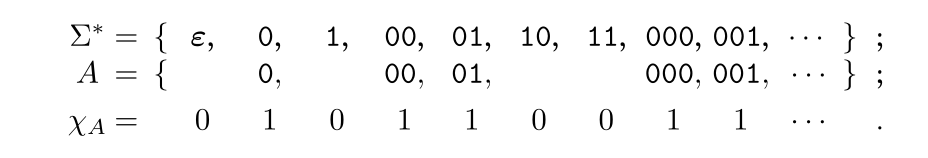
\includegraphics[scale=0.3]{figur/karsekv.png}
		      \end{center}

		\item Vi viser her et funktionen $f : \mathcal{L} \rightarrow \mathcal{B}$, hvor $f(A)$ er lig med den karakteristiske sekvens af $A$, er bijektiv. Derfor, da $\mathcal{B}$ er utællelig, er $\mathcal{L}$ også utællelig.
		\item Vi går nu tilbage til  sproget $A_{TM} = \{\langle M, w \rangle \mid M \text{ er en Turingmaskine og } M \text{ accepterer }w\}$
		\item Vi antager at $A_{TM}$ er afgørligt, og får dermed et modstrid.
		\item Antag at $H$ er en TM der afgører $A_{TM}$. På input $\langle M, w \rangle $, hvor $M$ er en TM og $w$ er en streng, stopper $H$ og accepterer hvis $M$ accepterer $w$. $H$ afviser hvis omvendt.
		\item Vi bruger nu $H$ til at konstruere en ny Turingmaskine, $D$, som bruger $H$.
		\item $D$ bruger $H$ til at bestemme hvad $M$ gør, hvis $M$ får sin egen beskrivelse, $\langle M \rangle$. Når den har fået denne information, gør den det omvendte.
		\item $D = $''På input \(\langle M \rangle \), hvor $M$ er en Turingmaskine:
		      \begin{enumerate}
			      \item Kør $H$ på input \(\langle M, \langle M \rangle \rangle\).
			      \item Output det omvendte af hvad $H$ outputter.
		      \end{enumerate}
		\item Det at $M$ kører med sig selv som input, bruges også i virkeligheden, for eksempel hvis en oversætter til Python i sig selv er skrevet i Python.

		\item Altså:
		      \begin{equation*}
			      D(\langle M \rangle ) = \begin{cases}
				      \text{\textit{accepter}} & \text{ hvis }M \text{ ikke accepterer } \langle M \rangle \\
				      \text{\textit{afvis}}    & \text{ hvis }M \text{ accepterer } \langle M \rangle
			      \end{cases}
		      \end{equation*}

		\item Hvad sker der så hvis vi kører $D$ på sin egen beskrivelse $\langle D \rangle $ som put? Så får vi:
		      \begin{equation*}
			      D(\langle M \rangle ) = \begin{cases}
				      \text{\textit{accepter}} & \text{ hvis }D \text{ ikke accepterer } \langle D \rangle \\
				      \text{\textit{afvis}}    & \text{ hvis }D \text{ accepterer } \langle D \rangle
			      \end{cases}
		      \end{equation*}
		\item Uanset hvad $D$ gør skal den gøre det omvendte, hvilket er umuligt. Dermed kan $D$ ikke eksisterer (og samme med $H$, da $D$ næsten eksklusivt bruger denne.)
	\end{itemize}
\end{frame}


\begin{frame}[allowframebreaks]
	\frametitle{Turing Ugenkendelighed}
	\begin{theorem}
		Et sprog $A$ er afgørligt $\iff$ $A$ er Turing-genkendeligt og co-Turing-genkendeligt
	\end{theorem}
	\begin{itemize}
		\item Her betyder co-Turing-genkendeligt, at dets komplement er Turing-genkendeligt.
		\item \(\Rightarrow\) Er tydeligt, hvis $A$ er afgørligt, er både $A$ og $\overline{A}$ også.
		\item \(\Leftarrow\) Vi konstsruerer en TM $M$:
		\item $M = $''På input $w$
		      \begin{enumerate}
			      \item Kør både $M_{1}$ og $M_{2}$ i parallel på input $w$
			      \item Hvis $M_{1}$ accepterer, så \textit{accepter}, hvis $M_{2}$ accepterer, så \textit{afvis}.''
		      \end{enumerate}
		\item Vi kan gøre dette, da vi ved at et genkendeligt sprog vil genkende alle strenge der er en del af $A$, men ikke nødvendigvis alle strenge der \textbf{ikke} er en del af $A$. Da $\overline{A}$ også er genkendeligt, kan vi strege dette over.
	\end{itemize}

	\begin{corollary}
		$\overline{A_{TM}}$ er ikke Turing-genkendeligt.
	\end{corollary}

	\begin{itemize}
		\item Vi ved at $A_{TM}$ er Turing-genkendeligt. Hvis $\overline{A_{TM}}$ også var Turing-genkendeligt, ville $A_{TM}$ være afgørligt.
	\end{itemize}
\end{frame}


\subsection{Uafgørlige Problemer fra Sprogteori}%
\label{subsec:uafgørligsprogteori}


\begin{frame}[allowframebreaks]
	\frametitle{Uafgørlige Problemer fra Sprogteori}
	\begin{itemize}
		\item Indtil videre har vi kun set ét uafgørligt problem.
		\item Vi vil nu få kigget på en del flere, herunder et af de mest kendte problemer i datalogi: Standsproblemet (halting problem).
		\item $HALT_{TM} = \{\langle M, w \rangle \mid M \text{ er en } TM \text{ og } M \text{ standser på input } w\}$
	\end{itemize}

	\begin{theorem}
		$HALT_{TM}$ er uafgørligt.
	\end{theorem}

	\begin{itemize}
		\item Vi bruger bevis ved modstrid.
		\item Vi gør dette ved at \textit{reducere} $A_{TM}$ til $HALT_{TM}$.
		\item I.e., vi beviser at hvis vi kan afgøre $HALT_{TM}$ kan vi \textbf{også} afgøre $A_{TM}$.
		\item Lad $R$ være en Turingmaskine der afgører $HALT_{TM}$ og lad $S$ være en Turingmaskine der afgører $A_{TM}$.
		\item $S = $''På input \(\langle M , w \rangle \), en kodning af en Turingmaskine $M$ og en streng $w$:
		      \begin{enumerate}
			      \item Kør $R$ på input \(\langle M , w \rangle\)
			      \item Hvis $R$ afviser, \textit{afvis}
			      \item Hvis $R$ accepterer, simulér $M$ på $w$ til den standser.
			      \item Hvis $M$ accepterer, \textit{accepter}, hvis $M$ afviser, \textit{afvis}.''
		      \end{enumerate}
		\item Altså kan vi bruge $HALT_{TM}$ til at afgøre $A_{TM}$.
		\item Vi går nu videre til tomhed i en Turingmaskine.
		\item $E_{TM} = \{\langle M \rangle \mid M \text{ er en Turingmaskine og }L(M) = \emptyset\}$
	\end{itemize}

	\begin{theorem}
		$E_{TM}$ er uafgørligt.
	\end{theorem}

	\begin{itemize}
		\item Lad $R$ være en TM der afgører $E_{TM}$.
		\item Vi bruger $R$ til at konsturere $S$ som afgører $A_{TM}$.
		\item Vi kører $R$ på en TM $M$ som vi modificerer til at afvise alle strenge undtagen $w$, som den kører på som normalt.
		\item Hvis $R$ accepterer denne, så ved vi $M$ \textbf{ikke} accepterer $w$, da sproget er tomt.
		\item Vi kalder den modificeret maskine $M_{1}$.
		\item $M_{1} = $ ``På input $x$:
		      \begin{enumerate}
			      \item Hvis $x \ne w$, \textit{afvis}.
			      \item Hvis $x = w$ kør $M$ på input $w$, og \textit{accepter} hvis $M$ accepterer.''
		      \end{enumerate}

		\item Vi antager at $R$ afgører $E_{TM}$ og konstruerer nu $S$ til at afgøre $A_{TM}$:
		\item $S = $''På input \(\langle M, w \rangle\), en kodning af en Turingmaskine $M$; og en streng $w$:
		      \begin{enumerate}
			      \item Brug beskrivelsen af $M$ og $w$ til at konstruere $M_{1}$.
			      \item Kør $R$ på input $\langle M_{1}\rangle$
			      \item Hvis $R$ accepterer, \textit{afvis}, hvis $R$ afviser, \textit{accepter}.''
		      \end{enumerate}
	\end{itemize}

	\begin{equation*}
		REGULAR_{TM} = \{\langle M \rangle \mid M \text{ er en Turingmaskine og } L(M) \text{ er et regulært sprog.}\}
	\end{equation*}

	\begin{theorem}
		$REGULAR_{TM}$ er uafgørligt
	\end{theorem}

	\begin{itemize}
		\item Vores idé her er at modificere $M$ således at $M_{2}$ (modificeret $M$) genkender et regulært sprog hvis og kun hvis $M$ accepterer $w$.
		\item Vi designer $M_{2}$ til at genkende det ikke-regulære sprog $\{0^{n}1^{n} \mid n \ge 0\}$ hvis $M$ \textbf{ikke} accepterer $w$, og genkende det regulære sprog $\Sigma^{*}$ hvis $M$ accepterer $w$.
		\item Bemærk at vi \textbf{ikke} konstruerer $M_{2}$ til rent faktisk at blive kørt!
		\item Vi konstruerer den udelukkende til at vise at $REGULAR_{TM}$ er umuligt.
		\item $S = $''På input \(\langle M, w \rangle\), hvor $M$ er en Turingmaskine og $w$ er en streng:
		      \begin{enumerate}
			      \item Konstruer den følgende Turingmaskine $M_{2}$:
			      \item[  ] $M_{2} =$''På input $x$:
			            \begin{enumerate}
				            \item Hvis $x$ er af formen $0^{n}1^{n}$, \textit{accepter}.
				            \item Hvis $x$ ikke har denne form, kør $M$ på input $w$  og \textit{accepter} hvis $M$ accepterer $w$.''
			            \end{enumerate}
			      \item Kør $R$ på input $\langle M_{2} \rangle $
			      \item Hvis $R$ accepterer, så \textit{accepter}, ellers \textit{afvis}.
		      \end{enumerate}
	\end{itemize}

	\begin{equation*}
		EQ_{TM} = \{\langle M_{1}, M_{2} \rangle \mid M_{1} \text{ og } M_{2} \text{ er Turingmaskiner og } L(M_{1}) = L(M_{2})\}
	\end{equation*}

	\begin{theorem}
		$EQ_{TM}$ er uafgørligt.
	\end{theorem}

	\begin{itemize}
		\item$S =$''På input \(\langle M \rangle \), hvor $M$ er en Turingmaskine:
		      \begin{enumerate}
			      \item Kør $R$ på input $\langle M, M_{1} \rangle$, hvor $M_{1}$ er en Turingmaskine der afviser alle input.
			      \item Hvis $R$ accepterer, \textit{accepter}, hvis $R$ afviser, \textit{afvis}.''
		      \end{enumerate}
		\item Her reducerer vi så fra $E_{TM}$ fremfor fra $A_{TM}$ som vi har gjort tidligere.
	\end{itemize}
\end{frame}



\subsection{Mapping Reducerbarhed}%
\label{subsec:mapping}

\begin{frame}[allowframebreaks]
	\frametitle{Mapping Reducerbarhed}
	\begin{itemize}
		\item Mapping reducerbarhed er blot reducerbarhed som vi har set tidligere, men formaliseret.
		\item Hvis vi kan reducere et problem $A$ til et problem $B$ ved at bruge mapping reducerbarhed, betyder det at en beregnelig funktion eksisterer, som konverterer instanser af problem $A$ til instanser af problem $B$.
		\item En sådan funktion  kan vi løse $A$ med en løser for $B$.
	\end{itemize}


	\begin{definition}[Beregnelig funktion]
		En funktion $f : \Sigma^{*} \longrightarrow \Sigma^{*}$ er en beregnelig funktion hvis en Turingmaskine $M$, på hvert input $w$, stopper med $f(w)$ på sit bånd.
	\end{definition}

	\begin{itemize}
		\item For eksempel er alle aritmetiske operationer beregnelige. For eksempel $f : \langle m , n \rangle \rightarrow m + n$ er beregnelig.
		\item Disse funktioner kan også være transformationer af maskinbeskrivelser.
		\item For eksempel kan en beregnlig funktion tage som input $w$ en turingmaskine $\langle M \rangle $ og returnere en modificeret maskine, $\langle M' \rangle $.
	\end{itemize}
\end{frame}

\begin{frame}[allowframebreaks]
	\frametitle{Formel Definition af Mapping Reducerbarhed}
	\begin{definition}
		Sprog $A$ er mapping reducerbart til sprog $B$, skrevet $A \le_{M} B$, hvis der er en beregnelig funktion $f : \Sigma^{*} \longrightarrow \Sigma^{*}$, hvor for hvert $w$,
		\begin{equation*}
			w \in A \iff f(w) \in B
		\end{equation*}

		Funktionen $f$ kaldes reduktionen fra $A$ til $B$.
	\end{definition}

	\begin{theorem}
		Hvis $A \le_{M} B$ og $B$ er afgørligt, så er $A$ afgørligt.
	\end{theorem}
	\begin{itemize}
		\item Lad $M$ være en afgører for $B$ og lad $f$ være reduktionen fra $A$ til $B$. Vi beskriver afgøreren $N$ for $A$ som følger:
		\item $N =$''På input $w$:
		      \begin{enumerate}
			      \item Beregn $f(w)$
			      \item Kør $M$ på input $f(w)$ og output hvad $M$ outputter.''
		      \end{enumerate}
		\item Så, hvis $w \in A$ så er $f(w) \in B$, og M accepterer $f(w)$ når $w \in A$.
		\item Følgende corollary har været det primære værktøj vi har brugt til at bevise uafgørlighed:
	\end{itemize}

	\begin{corollary}
		Hvis $A \le_{M} B$ og $A$ er uafgørligt, så er $B$ uafgørligt.
	\end{corollary}

	\begin{itemize}
		\item Vi kigger nu på nogle af vores tidligere eksempler, men med beregnelige funktioner.
		\item Vi viser nu en mapping reduktion fra $A_{TM}$ til $HALT_{TM}$.
		\item Vi præsenterer en beregnelig funktion $f : \langle M , w \rangle \rightarrow \langle M ' , w' )$, hvor
		      \begin{equation*}
			      \langle M , w \rangle \in A_{TM} \iff \langle M ', w' \rangle \in HALT_{TM}
		      \end{equation*}

		\item Følgende maskine $F$ beregner en reduktion $f$:
		\item $F =$''På input \(\langle M , w \rangle\):
		      \begin{enumerate}
			      \item Konstruér $M'$:. \\
			            $M' = $''På input $x$:
			            \begin{enumerate}
				            \item Kør $M$ på $x$
				            \item Hvis $M$ accepterer, \textit{accepter}
				            \item Hvis $M$ afviser, gå i løkke.''
			            \end{enumerate}
			      \item Output \(\langle M', w \rangle\)
		      \end{enumerate}
	\end{itemize}

	\begin{theorem}
		Hvis $A \le_{M} B$ og $B$ er Turing-genkendeligt, så er $A$ Turing-genkendeligt.
	\end{theorem}
	\begin{itemize}
		\item Beviset er det samme som ved afgørligt.
	\end{itemize}

	\begin{corollary}
		Hvis $A \le_{M} B$ og $A$ ikke er Turing-genkendeligt, så er $B$ ikke Turing-genkendeligt.
	\end{corollary}

	\begin{theorem}
		$EQ_{TM}$ er hverken Turing-genkendeligt eller co-Turing-genkendeligt.
	\end{theorem}
	\begin{itemize}
		\item Først viser vi at $EQ_{TM}$ ikke er Turing-genkendeligt.
		\item Vi viser dette ved at vise at $A_{TM} \le_{M} \overline{EQ_{TM}}$.
		\item Reduktionsfunktionen $f$ fungerer som følger:
		\item $F =$''På input \(\langle M, w \rangle\), hvor $M$ er en Turingmaskine og $w$ er en streng:
		      \begin{enumerate}
			      \item Konstruer følgende to maskiner: $M_{1}$ og $M_{2}$.\\
			            $M_{1} = $''På hvilket som helst input \textit{afvis}'' \\
			            $M_{2} =$''På hvilket som helst input, kør $M$ på $w$. \textit{Accepter} hvis den accepterer.\\
			      \item Output \(\langle M_{1}, M_{2} \rangle \)
		      \end{enumerate}
		\item Her accepterer $M_{1}$ intet.
		\item Hvis $M$ accepterer $w$, så accepterer $M_{2}$ \textbf{alt}.
		\item Dermed er de to maskiner \textbf{ikke} ens.
	\end{itemize}
\end{frame}




%%% Local Variables:
%%% mode: latex
%%% TeX-engine: xetex
%%% TeX-command-extra-options: "-shell-escape"
%%% TeX-master: "main"
%%% End:
